\section{Alternative Methoden}
\subsection{Mikrofonreihen} \label{ss:array}
Ein System bestehend aus mehreren Mikrofonen und Kameras ermöglicht eine sehr detaillierte Eventerkennung und räumlich Bewegungsverfolgung von Objekten und Personen im überwachten Bereich. Das in \cite{Che02} beschriebene System überwacht einen Konferenzsaal mit 32 ungerichteten Mikrofonen, welche an der Decke des Saales befestigt sind, und zwei Videokameras ähnlich zu der in Abbildung \ref{FIG:Array:Setup} dargestellten Umgebung.

\begin{figure}
\centering
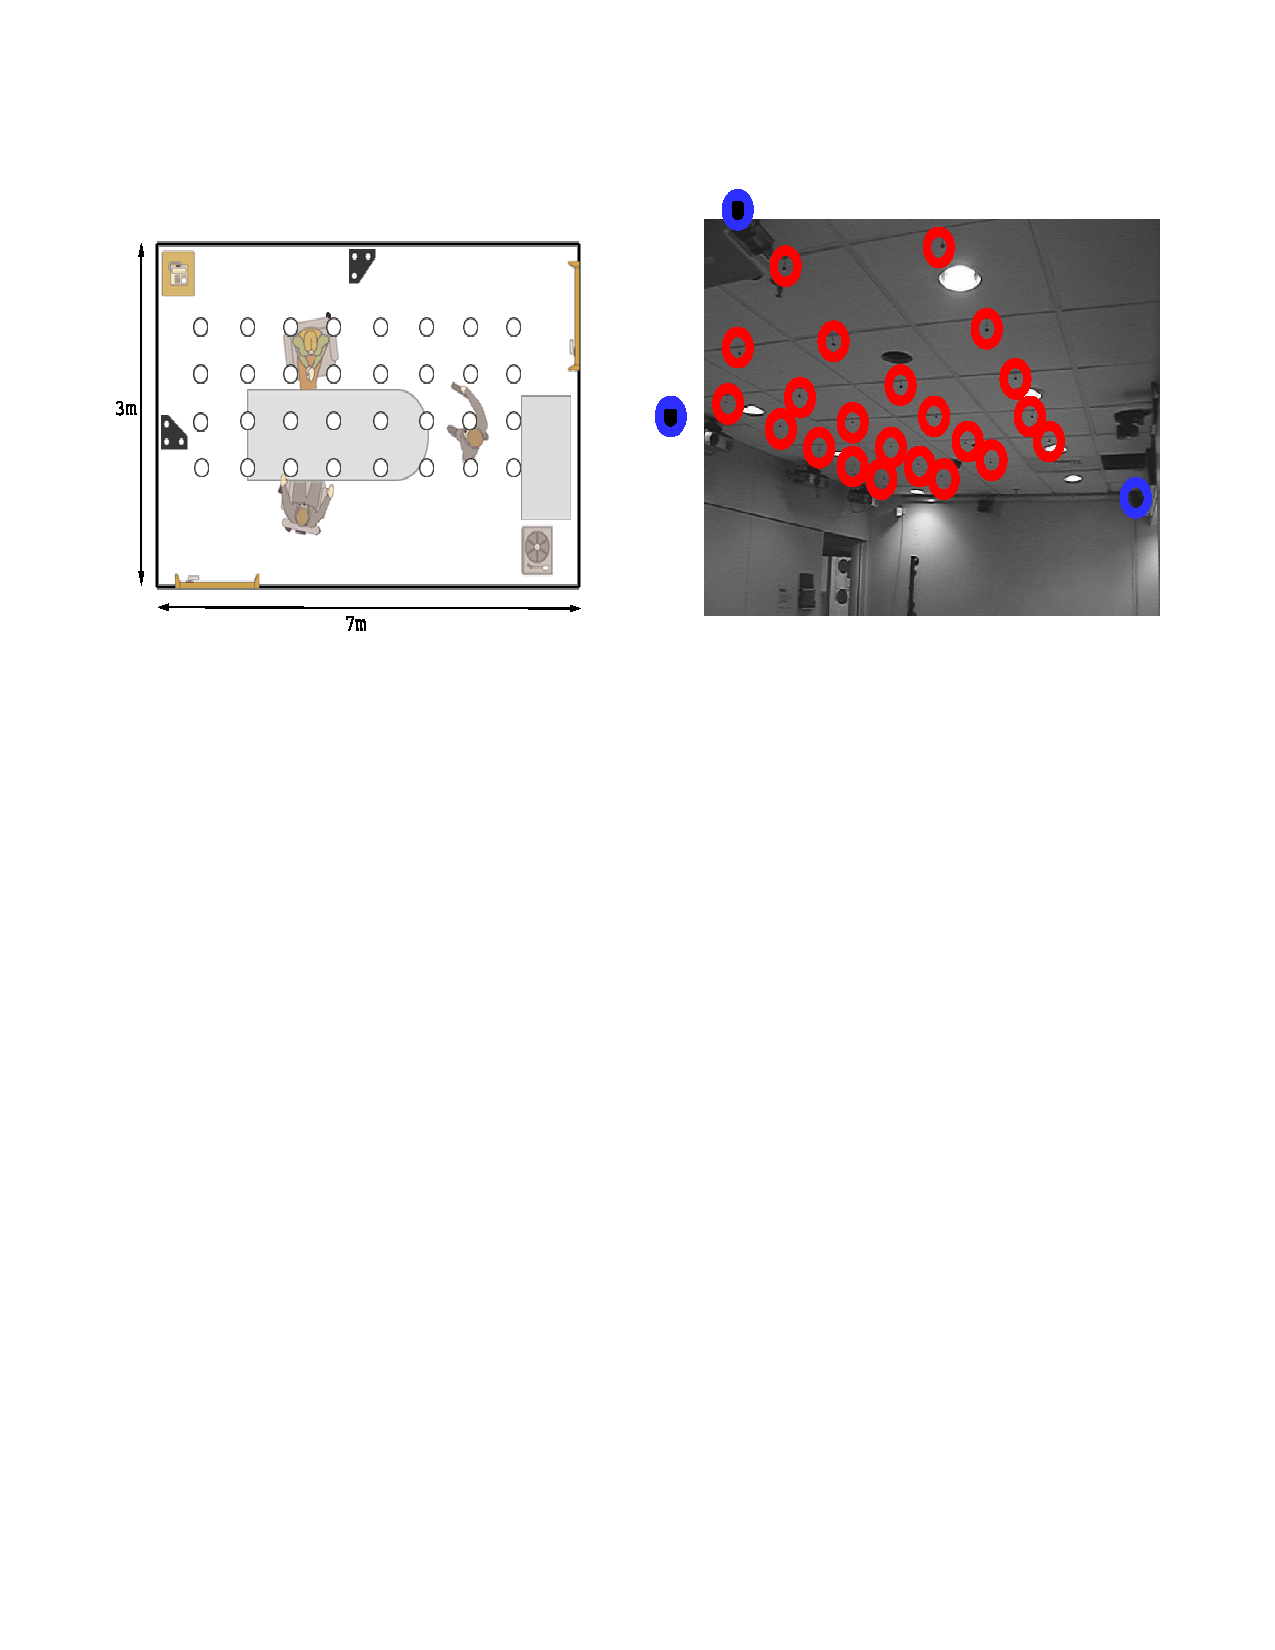
\includegraphics[width=\linewidth]{\figdir//MA-Setup.pdf}
\caption{Links eine schematische Zeichnung, in der die Kreise Mikrofone darstellen und die schwarzen Dreiecke Kameras. Rechts ist ein Foto der Testumgebung in welchem Kameras und Mikrofone hervorgehoben wurden. Quelle \cite{Array:Setup}}
\label{FIG:Array:Setup}
\end{figure}

Die Videoaufnahmen werden mit einer Foreground-Background-Analysis aufbereitet um Veränderungen in den Aufnahmen kenntlich zu machen. Diese Veränderungen im Verhältnis zur Zeit stellen die Bewegungen der Personen in den Videoaufnahmen dar \cite{Array:Video}. Da die Anwendung Personen in einem Konferenzsaal beobachtet, wird die Position lediglich auf eine zweidimensionalen Fläche projiziert. In Abbildung \ref{FIG:Array:Video} ist eine Videoanalyse zu sehen. Die X und Y Achsen geben die Position der Bewegung im Raum an während die Z Achse der zeitliche Verlauf ist. In der Abbildung ist eine Momentaufnahme für t=29 zu sehen. Diese zeigt alle Regionen, in denen zu diesem Zeitpunkt t Bewegungen festgestellt wurden. Insgesamt zeigt die Grafik einen Bewegungsverlauf von zwei Personen, welche sich der Raummitte nähern und einem Objekt in der Raummitte, welches ungefähr ab dem Zeitpunkt t=25 bewegt wird. Nach dem Zeitpunkt t=40 bewegen sich die zwei Personen wieder aus der Mitte des Raumes hinaus.

\begin{figure}
\centering
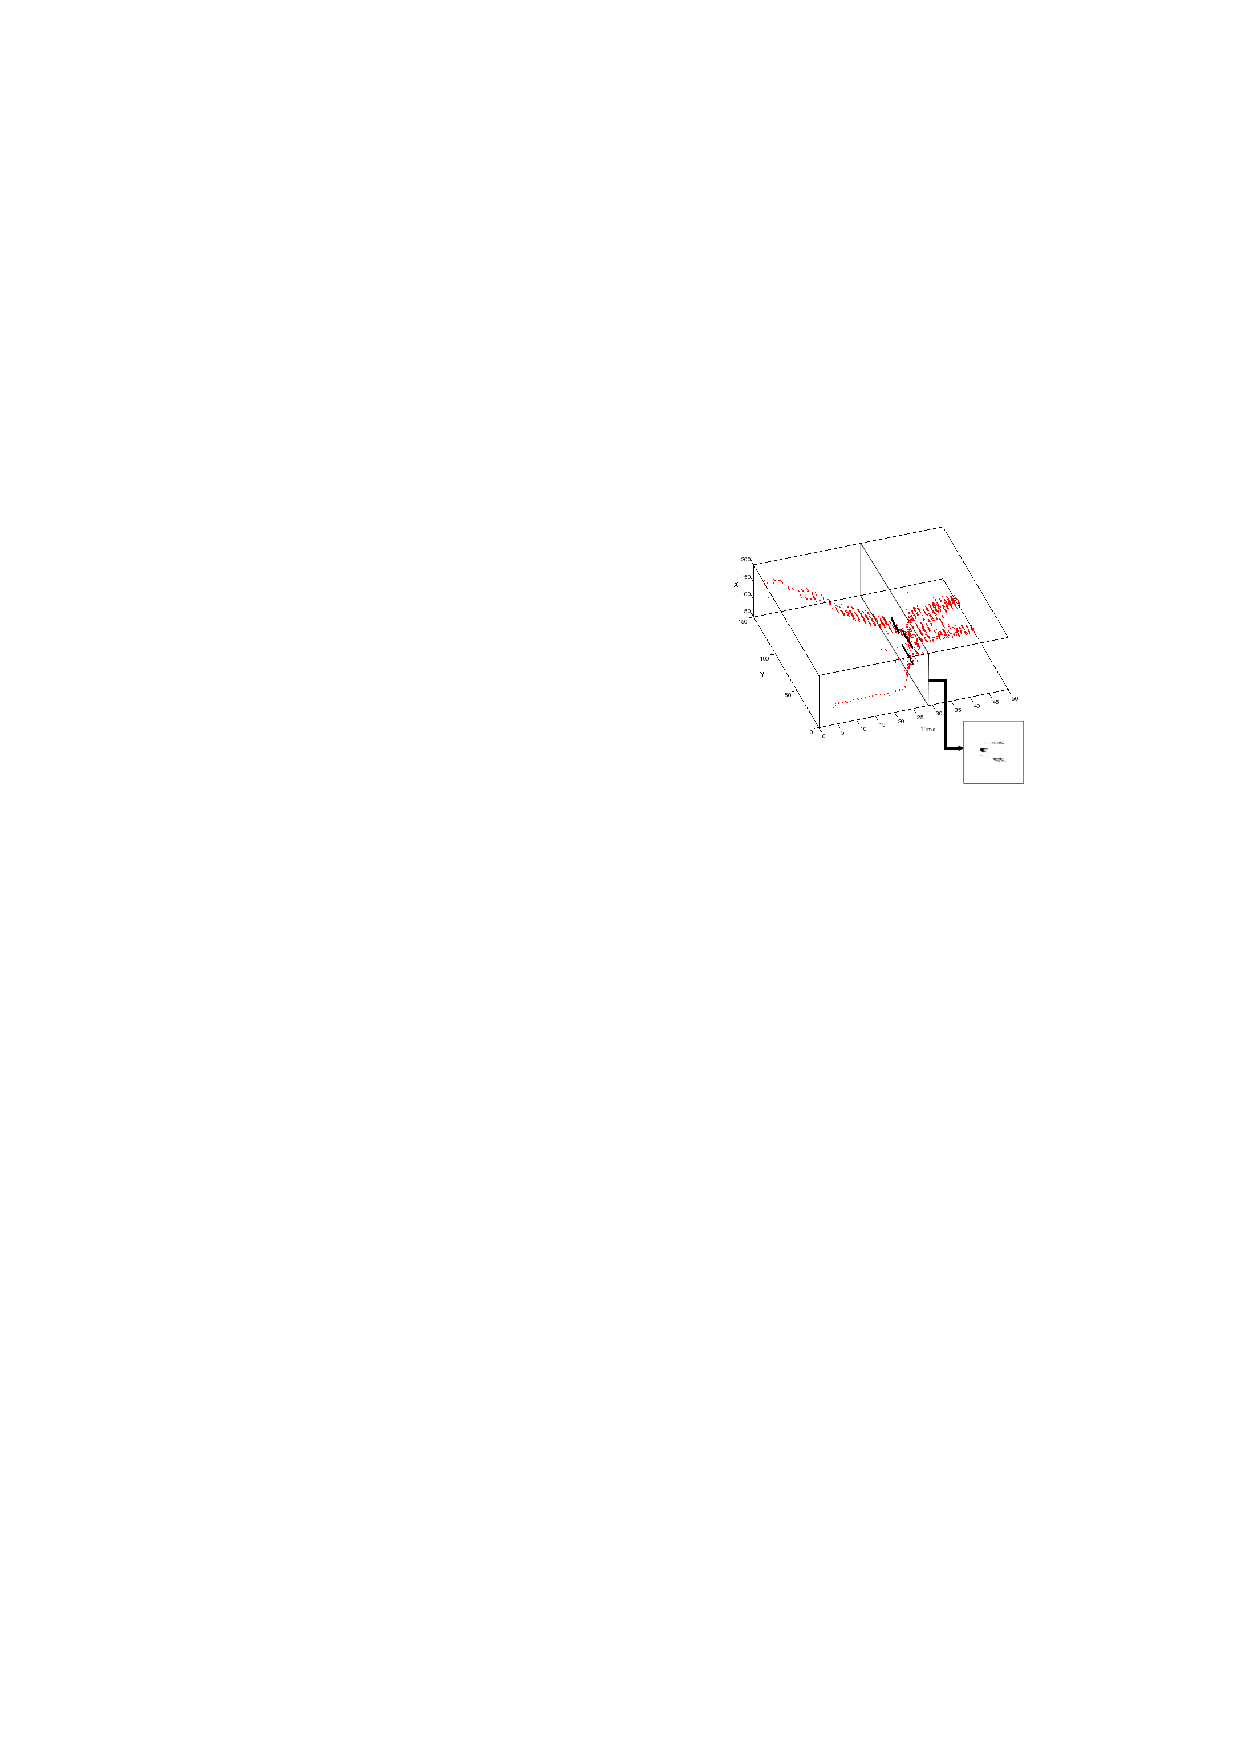
\includegraphics[width=0.75\linewidth]{\figdir//MA-VT.pdf}
\caption{Video Analyse von Bewegungen im Verlauf der Zeit}
\label{FIG:Array:Video}
\end{figure}

Mit den Werten der Mikrofone wird die Lautstärke im Vergleich zu Rauschgeräuschen (SNR, Signal-Noise-Ratio) auf dem Raum abgebildet. Somit wird ein Graph wie in Abbildung \ref{FIG:Array:Audio} erzeugt. Da dieses System eine Gruppe von Menschen beobachtet, arbeitet es unter der Annahme, dass Bewegung und Geräusche korrelieren. Deshalb werden die Positionen, an denen es visuelle Bewegungen gab, als Ausgangspunkt für eine Suche nach einem lokalen Maximum im Audiographen verwendet \cite{Che02:Audio}. Somit kann die genaue Position der Geräuschquelle lokalisiert werden. Mithilfe der Position können die Zeitverzögerungen der Audioaufnahmen der unterschiedlichen Mikrofone berechnet und somit das Zielgeräusch von Hintergrundgeräuschen getrennt werden \cite{Array:Audio}.    

\begin{figure}
\centering
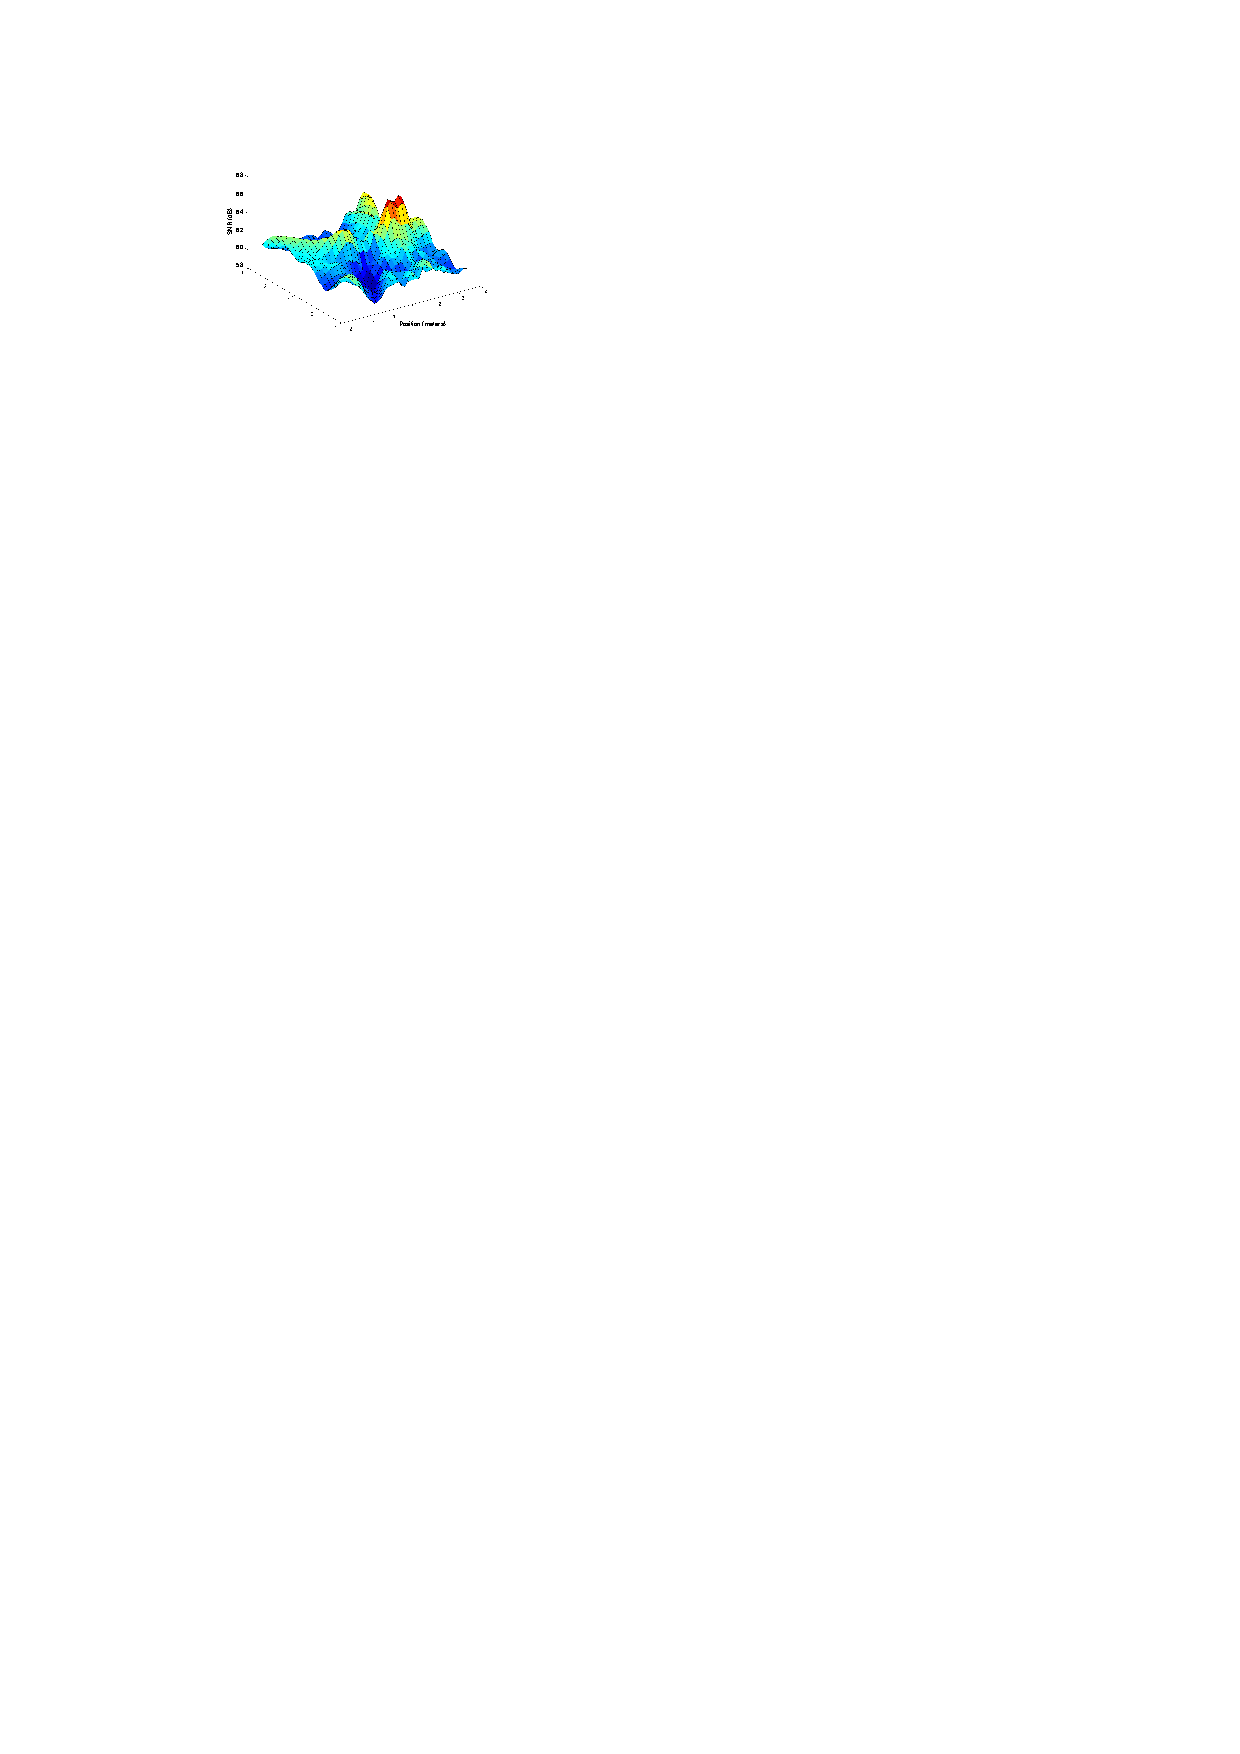
\includegraphics[width=0.8\linewidth]{\figdir//MA-AT.pdf}
\caption{Räumliche Audio Analyse durch mehrere Mikrofone}
\label{FIG:Array:Audio}
\end{figure}

\bigskip

Die Audio- und Videodaten werden zu einem beobachteten Zustand \textit{z} kombiniert. Dann wird berechnet wie wahrscheinlich diese Beobachtung \textit{z} für eine hypothetische Konfiguration \textit{O\textsubscript{t}}
\begin{equation}
O_t = (o_1, ..., o_n)
\end{equation}

aus \textit{n} Objekten zum Zeitpunkt \textit{t} ist, wobei \textit{O\textsubscript{i} = [x, y, h, f]} der Zustandsvektor eines Objektes ist. Hierbei werden Personen als Zylinder der Höhe \textit{h} mit festgelegten Radio dargestellt, dessen Position auf dem Boden durch [\textit{x, y}] dargestellt wird. \textit{f} ist die Frequenz ihrer Stimme.

Für ein einzelnes Objekt gibt \textit{L(z|O\textsubscript{i})} an, wie wahrscheinlich die Hypothese eines einzelnen Objektes von der Beobachtung unterstützt wird. Dies wird berechnet aus

\begin{equation}
L(z|o_i) = L(z_a|o_i) * L(z_v|o_i)
\end{equation}

wobei $L(z_a|o_i)$ und $L(z_v|o_i)$ angeben, wie sehr die Audio- beziehungsweise Videodaten die Hypothese $o_i$ unterstützen.

Die Wahrscheinlichkeit $L_t(z|O)$, dass der beobachtete Zustand für eine Hypothese \textit{O} bestehend aus \textit{m} Objekten auftritt lässt sich mit dem gauschen Fehlintegral aus den Einzelwahrscheinlichkeiten der Objekte berechnen

\begin{equation}
L_t(z|O) = \phi L(z|o_1), ..., L(z|o_m)
\end{equation}

\bigskip

Mikrofonreihen erlauben es selbst sich bewegende Audio-Visuelle Ereignisse mit einer Genauigkeit von bis zu 10 Zentimeter zu erkennen und verfolgen. Somit können auch Gespräche zwischen zwei nahestehenden Personen korrekt erkannt werden. Auch können zwei gleichzeitige, unabhängige AV Events separat erkannt werden. Jedoch benötigt diese Methode eine große Menge an Mikrofonen und Rechenleistung und ist daher nur in sehr kontrollierten Umgebungen einsetzbar \cite{Che02}.

\subsection{Dualmikrofon mit HHM}

\subsection{Cononical correlation analysis}

\subsection{Maximization of mutual information}

\subsection{Computational Auditory Scene Analysis CASA}
\subsection{Computational Auditory Scene Recognition CASR}
